\section{Benchmark NIST-8 "Oscillatory"}
\label{sec:bench-8}

This is a wave function that satisfies the Schr\"{o}dinger's equation model of two
interacting atoms, highly oscillatory near the origin.
The equation solved in this problem is the Helmholtz equation.

\begin{equation} \label{oscillatory}
-\nabla^{2} u - \frac{1}{(\alpha + r)^{4}} u = f
\end{equation}

in the domain $\Omega = (0, 1)^2$, equipped with Dirichlet boundary conditions
given by the exact solution. The exact solution:

\begin{equation}\label{exact-nist-8}
u(x,y) = sin(\frac{1}{\alpha + r})
\end{equation}

where $r = \sqrt{x^{2} + y^{2}}$, $\alpha = 1 / N \pi$ determines the number of oscillations.
The right-hand side $f$ is calculated by inserting (\ref{exact-nist-8}) into (\ref{oscillatory}).
The solution of NIST-8 with $\alpha = 1 / 10 \pi$ is shown in Fig. \ref{fig:sln-nist08}.

\begin{figure}[!ht]
\centering
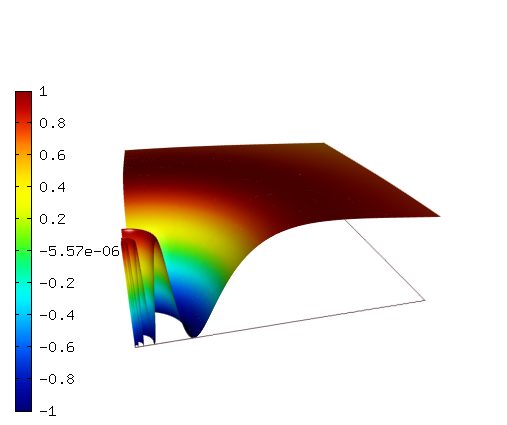
\includegraphics[height=6cm]{nist/nist-8/solution.png}
\caption{The solution to NIST-8 benchmark problem.}
\label{fig:sln-nist08}
\end{figure}

The goal of the benchmark is to reach a relative error below
$10^{-2}$~\% in the $H^1$-norm with as few DOFs as possible.
We begin with adaptive $hp$-FEM,
the initial mesh is shown in Fig. \ref{fig:nist-8-hp-aniso} (left).
After 28 adaptivity steps, the resulting mesh with 1160 DOF is shown
in Fig. \ref{fig:nist-8-hp-aniso} (right).

\begin{figure}[!ht]
\centering
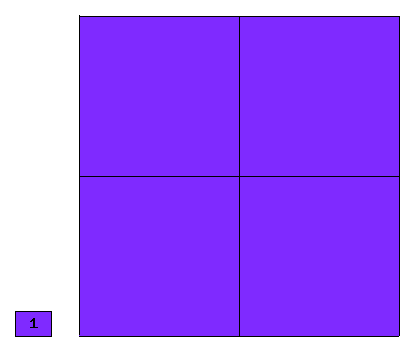
\includegraphics[height=5cm]{nist/nist-8/mesh_hp_aniso_init.png}\ \
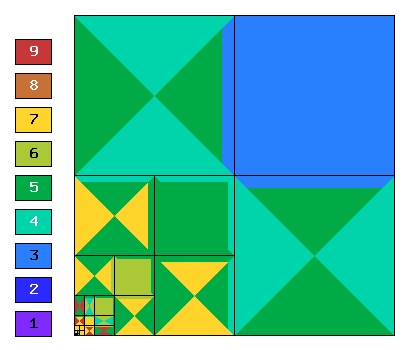
\includegraphics[height=5cm]{nist/nist-8/mesh_hp_aniso.png}
\caption{Initial mesh (left) and final mesh (right) for $hp$-FEM with anisotropic refinements.}
\label{fig:nist-8-hp-aniso}
\end{figure}

The final relative error estimate in $H^1$-norm was 9.09848e-02 \%,
and it was identical to the exact error in all printed digits.
We also solved this benchmark with adaptive $h$-FEM
with linear (left) and quadratic (right)
elements, with anisotropic refinements enabled.
Final meshes for the $h$-FEM computations are shown
in Fig. \ref{fig:nist-8-h-aniso}.

\begin{figure}[!ht]
\centering
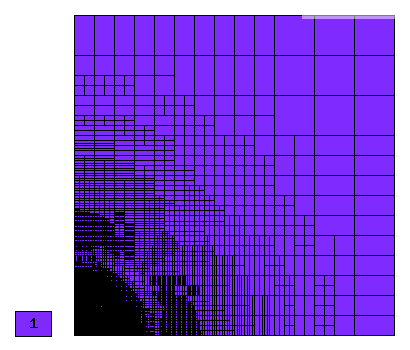
\includegraphics[height=5cm]{nist/nist-8/mesh_h1_aniso.png}\ \
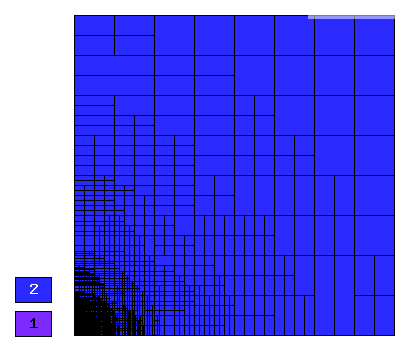
\includegraphics[height=5cm]{nist/nist-8/mesh_h2_aniso.png}
\caption{Final mesh for $h$-FEM anisotropic refinements with linear and quadratic elements.}
\label{fig:nist-8-h-aniso}
\end{figure}

Finally, Figs. \ref{fig:nist-8-conv} compare all
three approaches to automatic adaptivity from the point
of view of DOF and CPU convergence.

\begin{figure}[!ht]
\centering
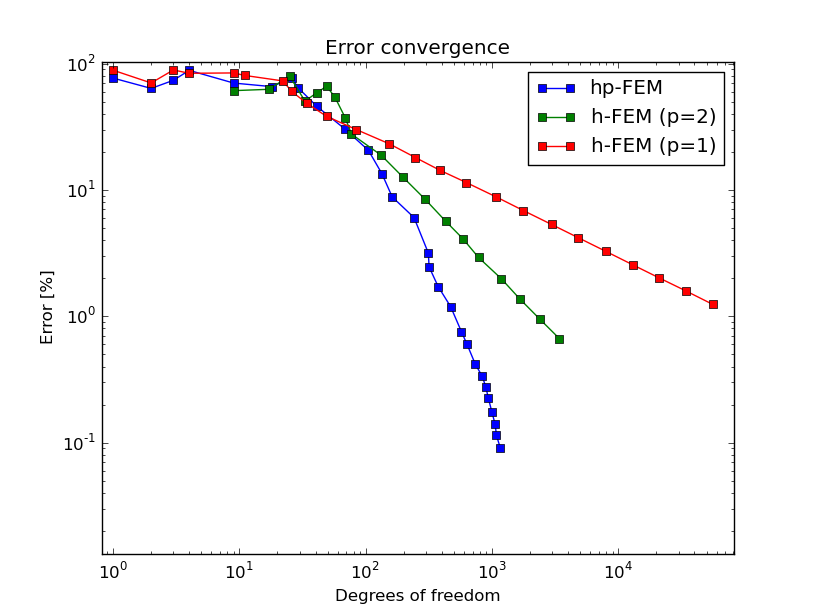
\includegraphics[height=5cm]{nist/nist-8/conv_dof_aniso.png}\ \
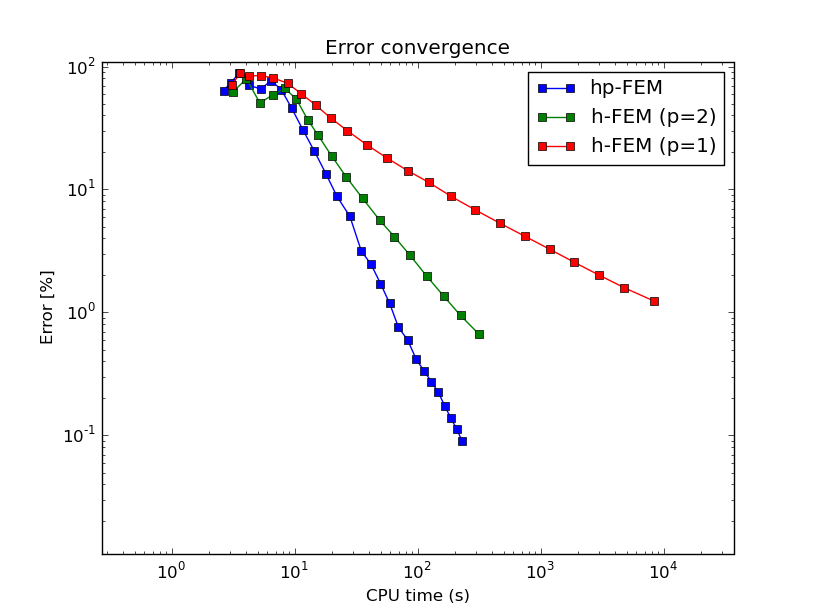
\includegraphics[height=5cm]{nist/nist-8/conv_cpu_aniso.png}
\caption{DOF and CPU time convergence graphs.}
\label{fig:nist-8-conv}
\end{figure}

